\section{Cấu trúc gói tin}

Gradient Server Model định nghĩa hai loại gói tin chính để thực hiện chức năng định tuyến: GRADIENT\_STATUS dùng để trao đổi thông tin gradient giữa các node, và DATA dùng để chuyển tiếp dữ liệu ứng dụng về sink node. Các gói tin này được thiết kế tối giản để phù hợp với giới hạn payload của BLE Mesh, đồng thời chứa đủ thông tin cần thiết cho việc định tuyến.

\subsection{Định nghĩa Opcode}

Trong BLE Mesh, mỗi loại message được định danh bằng một opcode. Đối với Vendor Model như Gradient Server Model, opcode có độ dài 3 bytes, bao gồm 1 byte định danh vendor opcode (0xC0-0xFF) và 2 bytes Company ID. Gradient Server Model sử dụng Company ID của Nordic Semiconductor (0x0059) và định nghĩa các opcode như sau:

\begin{table}[h!]
\centering
\caption{Định nghĩa Opcode cho Gradient Server Model}
\label{tab:gradient_opcodes}
\begin{tabular}{|l|l|p{8cm}|}
\hline
\textbf{Opcode} & \textbf{Tên} & \textbf{Mô tả} \\
\hline
0x0A & GRADIENT\_STATUS & Gói tin broadcast chứa thông tin gradient của node gửi. Được sử dụng để thiết lập và duy trì giá trị gradient trong mạng. \\
\hline
0x0B & DATA & Gói tin unicast chứa dữ liệu thu thập từ cảm biến, được chuyển tiếp theo hướng gradient giảm dần về sink node. \\
\hline
\end{tabular}
\end{table}

Việc sử dụng vendor opcode (thay vì SIG opcode) cho phép Gradient Server Model hoạt động độc lập với các SIG Model chuẩn, tránh xung đột opcode và đảm bảo tính tương thích với các thiết bị BLE Mesh từ nhiều nhà sản xuất khác nhau.

\subsection{Gói tin GRADIENT\_STATUS}

Gói tin GRADIENT\_STATUS được sử dụng để broadcast thông tin gradient của một node đến tất cả các node lân cận trong phạm vi phủ sóng. Đây là gói tin cốt lõi trong cơ chế thiết lập và duy trì gradient, được gửi định kỳ bởi mỗi node và khi có sự thay đổi gradient.

\subsubsection{Cấu trúc gói tin}

Gói tin GRADIENT\_STATUS được đóng gói trong BLE Mesh Network PDU với cấu trúc như sau:

\begin{figure}[h!]
    \centering
    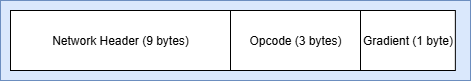
\includegraphics[width=0.75\textwidth]{chapter3/image/Gradient_Status.png}
    \caption{Cấu trúc gói tin GRADIENT\_STATUS}
    \label{fig:gradient_status_packet}
\end{figure}

Cấu trúc gói tin GRADIENT\_STATUS bao gồm hai phần chính: Network Header và Application Payload. Network Header có kích thước 9 bytes theo chuẩn BLE Mesh, chứa các trường thông tin cần thiết cho việc định tuyến và bảo mật ở lớp Network. Cụ thể, byte đầu tiên chứa IV Index (1 bit) và Network ID (7 bits) dùng để xác định khóa giải mã gói tin. Byte thứ hai chứa Control flag (1 bit) phân biệt giữa control message và access message, cùng với Time To Live (7 bits) quy định số hop tối đa mà gói tin có thể đi qua - giá trị mặc định là 10 cho broadcast. Ba bytes tiếp theo là Sequence Number, tăng dần sau mỗi gói tin để chống replay attack và đảm bảo tính duy nhất của message. Hai bytes SRC chứa địa chỉ unicast của node gửi gói tin, trong khi hai bytes DST chứa địa chỉ đích - thường là group address 0xFFFF cho trường hợp broadcast đến tất cả node trong mạng.

Phần Application Payload của GRADIENT\_STATUS rất gọn nhẹ, chỉ bao gồm 3 bytes Opcode (0x0A) để định danh loại gói tin, và 1 byte Gradient Value chứa giá trị gradient của node gửi. Giá trị gradient nằm trong khoảng 0 đến 255, trong đó 0 biểu thị sink node và 255 biểu thị node chưa có kết nối hợp lệ đến sink. Thiết kế payload tối giản này giúp giảm thiểu overhead truyền thông và phù hợp với giới hạn kích thước của BLE advertising packet.

\subsection{Gói tin DATA}

Gói tin DATA được sử dụng để truyền dữ liệu ứng dụng (sensor data, control commands, ...) từ các node trong mạng về sink node. Khác với GRADIENT\_STATUS được broadcast, gói tin DATA sử dụng unicast addressing để chuyển tiếp qua từng hop theo hướng gradient giảm dần.

\subsubsection{Cấu trúc gói tin}

\begin{figure}[h!]
    \centering
    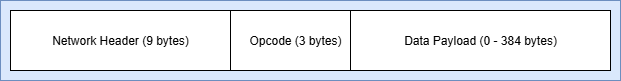
\includegraphics[width=0.75\textwidth]{chapter3/image/Data.png}
    \caption{Cấu trúc gói tin DATA}
    \label{fig:data_packet}
\end{figure}

Cấu trúc gói tin DATA tương tự như GRADIENT\_STATUS, bao gồm Network Header, vàApplication Payload. Network Header có kích thước 9 bytes theo chuẩn BLE Mesh, chứa đầy đủ các trường IVI, NID, CTL, TTL, SEQ, SRC và DST để đảm bảo việc định tuyến và bảo mật ở lớp Network. Điểm khác biệt quan trọng là trường DST trong gói tin DATA chứa địa chỉ unicast của next-hop thay vì group address, vì gói tin được chuyển tiếp hop-by-hop theo hướng gradient giảm dần.

Phần Application Payload của gói tin DATA bao gồm ba thành phần chính. Đầu tiên là 3 bytes Opcode (0x0B) để định danh loại gói tin DATA. Sau đó là Payload chứa dữ liệu thu thập từ cảm biến thực tế. Kích thước Payload tối đa là 6 bytes cho unsegmented message; với các ứng dụng cần truyền lượng dữ liệu lớn hơn, BLE Mesh hỗ trợ segmented message cho phép payload lên đến 384 bytes thông qua cơ chế phân mảnh và tái hợp ở lớp Lower Transport.
